Необходимость применения методов компьютерного зрения в рамках данной работы обусловлена тем, что автоматизация обработки документов требует не только распознавания текста, но и предварительного анализа изображения документа. Как показано в работе А.~Р.~Давлетова~\cite{refDavletov}, современные системы решают задачи предварительной обработки изображения, обнаружения текстовых областей, анализа компоновки страницы и последующего распознавания символов и слов. Такой подход позволяет преобразовывать сканированные документы, PDF-файлы и изображения, полученные при сканировании, в машинно-обрабатываемый текст, пригодный для поиска, редактирования и дальнейшего извлечения данных~\cite{refDavletov}. 

По сравнению с ручной обработкой автоматизированный подход сокращает время ввода данных, снижает влияние человеческого фактора, уменьшает количество ошибок и упрощает поиск и доступ к информации~\cite{refDavletov}. 

% Кроме того, в рассматриваемой статье отмечается, что применение методов машинного обучения совместно с OCR позволяет не только конвертировать изображение в текст, но и извлекать из него полезные данные, а в практических сценариях такие решения демонстрируют высокую точность и значительный уровень автоматизации документооборота~\cite{refDavletov}.


\begin{figure*}[hbtp]
	\centering
	\begin{tabular}{cc}
		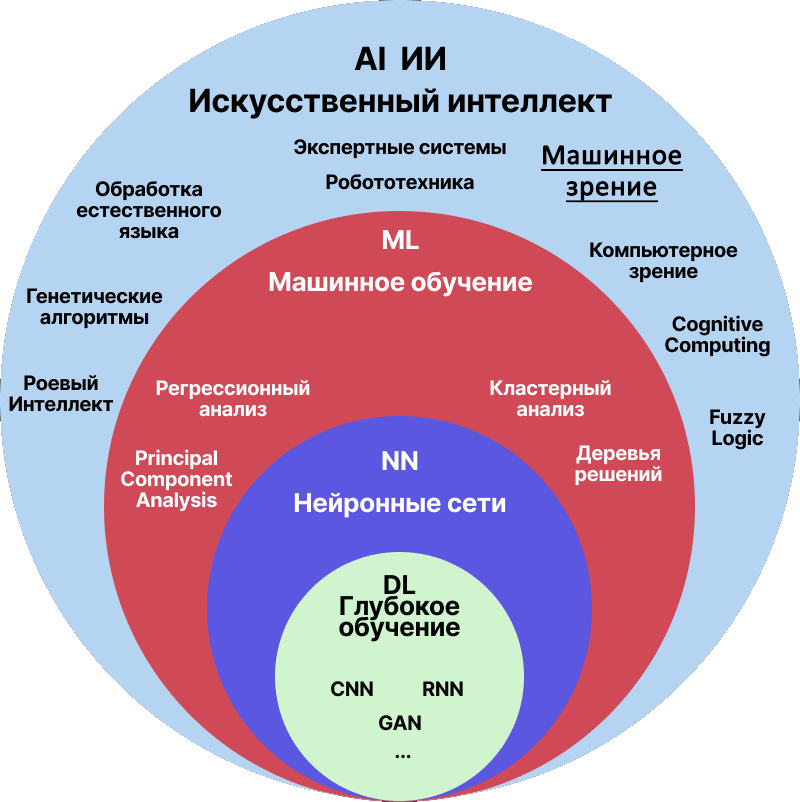
\includegraphics[width=0.45\linewidth]{img/classifications_ai.png} &
		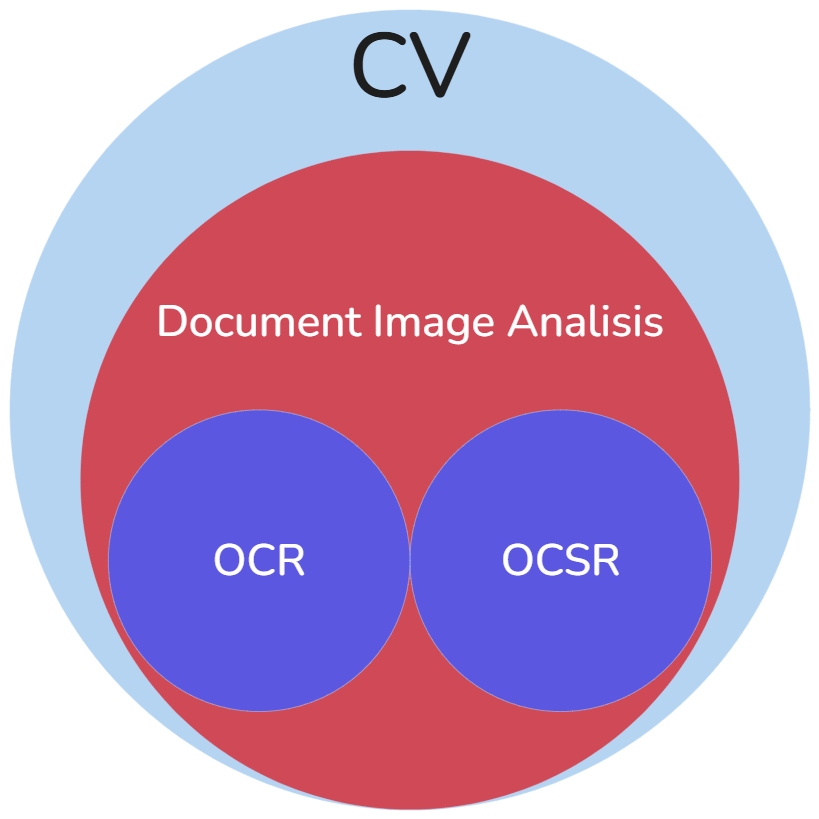
\includegraphics[width=0.45\linewidth]{img/classifications_cv.png} \\
		a$)$ & b$)$
	\end{tabular}
	\bicaption
	{
		а) Классификация искусственного интеллекта;
		b) Классификация компьютерного зрения.
	}
	{
		a) Classification of artificial intelligence;
		b) Classification of computer vision.
	}
	\label{fig:classifications_ai}
\end{figure*}
